\documentclass[a4paper,12pt]{scrreprt}

\usepackage[english]{babel}
\usepackage[utf8x]{inputenc}
\usepackage{ucs}

\usepackage{hyperref}

\usepackage{graphicx}
\usepackage{float}

\title{Kingdom of Kush - 0 A.D. Mod - Specification}

\begin{document}

\maketitle

\abstract{This is the development specification for the Kushite Mod. The Kushite Mod adds the Kushite civilization to the real time strategy game \href{https://play0ad.com/}{0 A.D.}.}

\tableofcontents

\chapter{Units, Buildings and Technology Tree}

Buildings:

\begin{itemize}
	\item Temple
	\item Civic Center
	\item Storage Depot $\rightarrow$ TODO Research \& Sketch
	\item House
	\item Blacksmith $\rightarrow$ TODO Sketch
	\item Fields
	\item Farmstead
	\item Stable
	%\item (TODO Something like a Mill)
	\item Marketplace $\rightarrow$ TODO Sketch
	\item Trader (land)
	\item Fishing Boat $\rightarrow$ TODO Research (papyrus or wooden?) \& Sketch
	\item Light Warship
	\item Medium Warship
	\item Dock
	\item Diplomacy Center $\rightarrow$ TODO Research (where/how did they hire mercenaries?)
	\item Garrison/Barrack $\rightarrow$ TODO Research (how did they look like?)
	\item Fortress
	\item Tower
	\item Wall
	\item Wonder
\end{itemize}

Units:

\begin{itemize}
	\item Woman worker $\rightarrow$ TODO Research (how did they look like? Avoid racial bias)
	\item Basic infantry/cavalry workers $\rightarrow$ TODO Research (how did they look like?)
	\item Chariots
	\item Beja Swordsman (mercenaries)
	\item Beja Camel Warrior (mercenaries)
	\item Siege Weapons
	\begin{itemize}
		\item Battering Ram
		\item Siege Tower
	\end{itemize}
	\item Elite Units
	\begin{itemize}
		\item Nubian Bowmen
		\item TODO other elite units
	\end{itemize}
	\item Heros $\rightarrow$ TODO Research (Important Queens/Kings, Priests etc.)
	\begin{itemize}
		\item Arikhankharer TODO Research \& Decision
		\begin{itemize}
			\item With the ability to recruit 1 to 5 dogs which automatically guard him (like in AOEIII) would be an interesting idea. Because of the dogs, any unit within his area of influence would get a defense bonus.  
		\end{itemize}
	\end{itemize}
\end{itemize}

Special Technologies:

\begin{itemize}
	\item Iron production bonus
	\item Cattle bonus
\end{itemize}

Agriculture:

\begin{itemize}
	\item Wheat fields
	\item Animals
	\begin{itemize}
		\item Sanga Cattle
		\item Goat
	\end{itemize}
\end{itemize}
Special Features:

\begin{itemize}
	\item Nubian Bowmen shoot poisoned arrows
\end{itemize}

\section{Buildings}

\subsection{Temple}

\subsection{Civic Center}

\subsection{Storage Depot}

\subsection{House}

\paragraph{About the Common House \ref{fig:common_house}:} Looks quite Kushite. The large ceramic pot, fixed in the floor in the corner of the courtyard is very good. I saw pictures of that in archeological digs of Meroitic sites.

\begin{figure}[H]
	\centering
	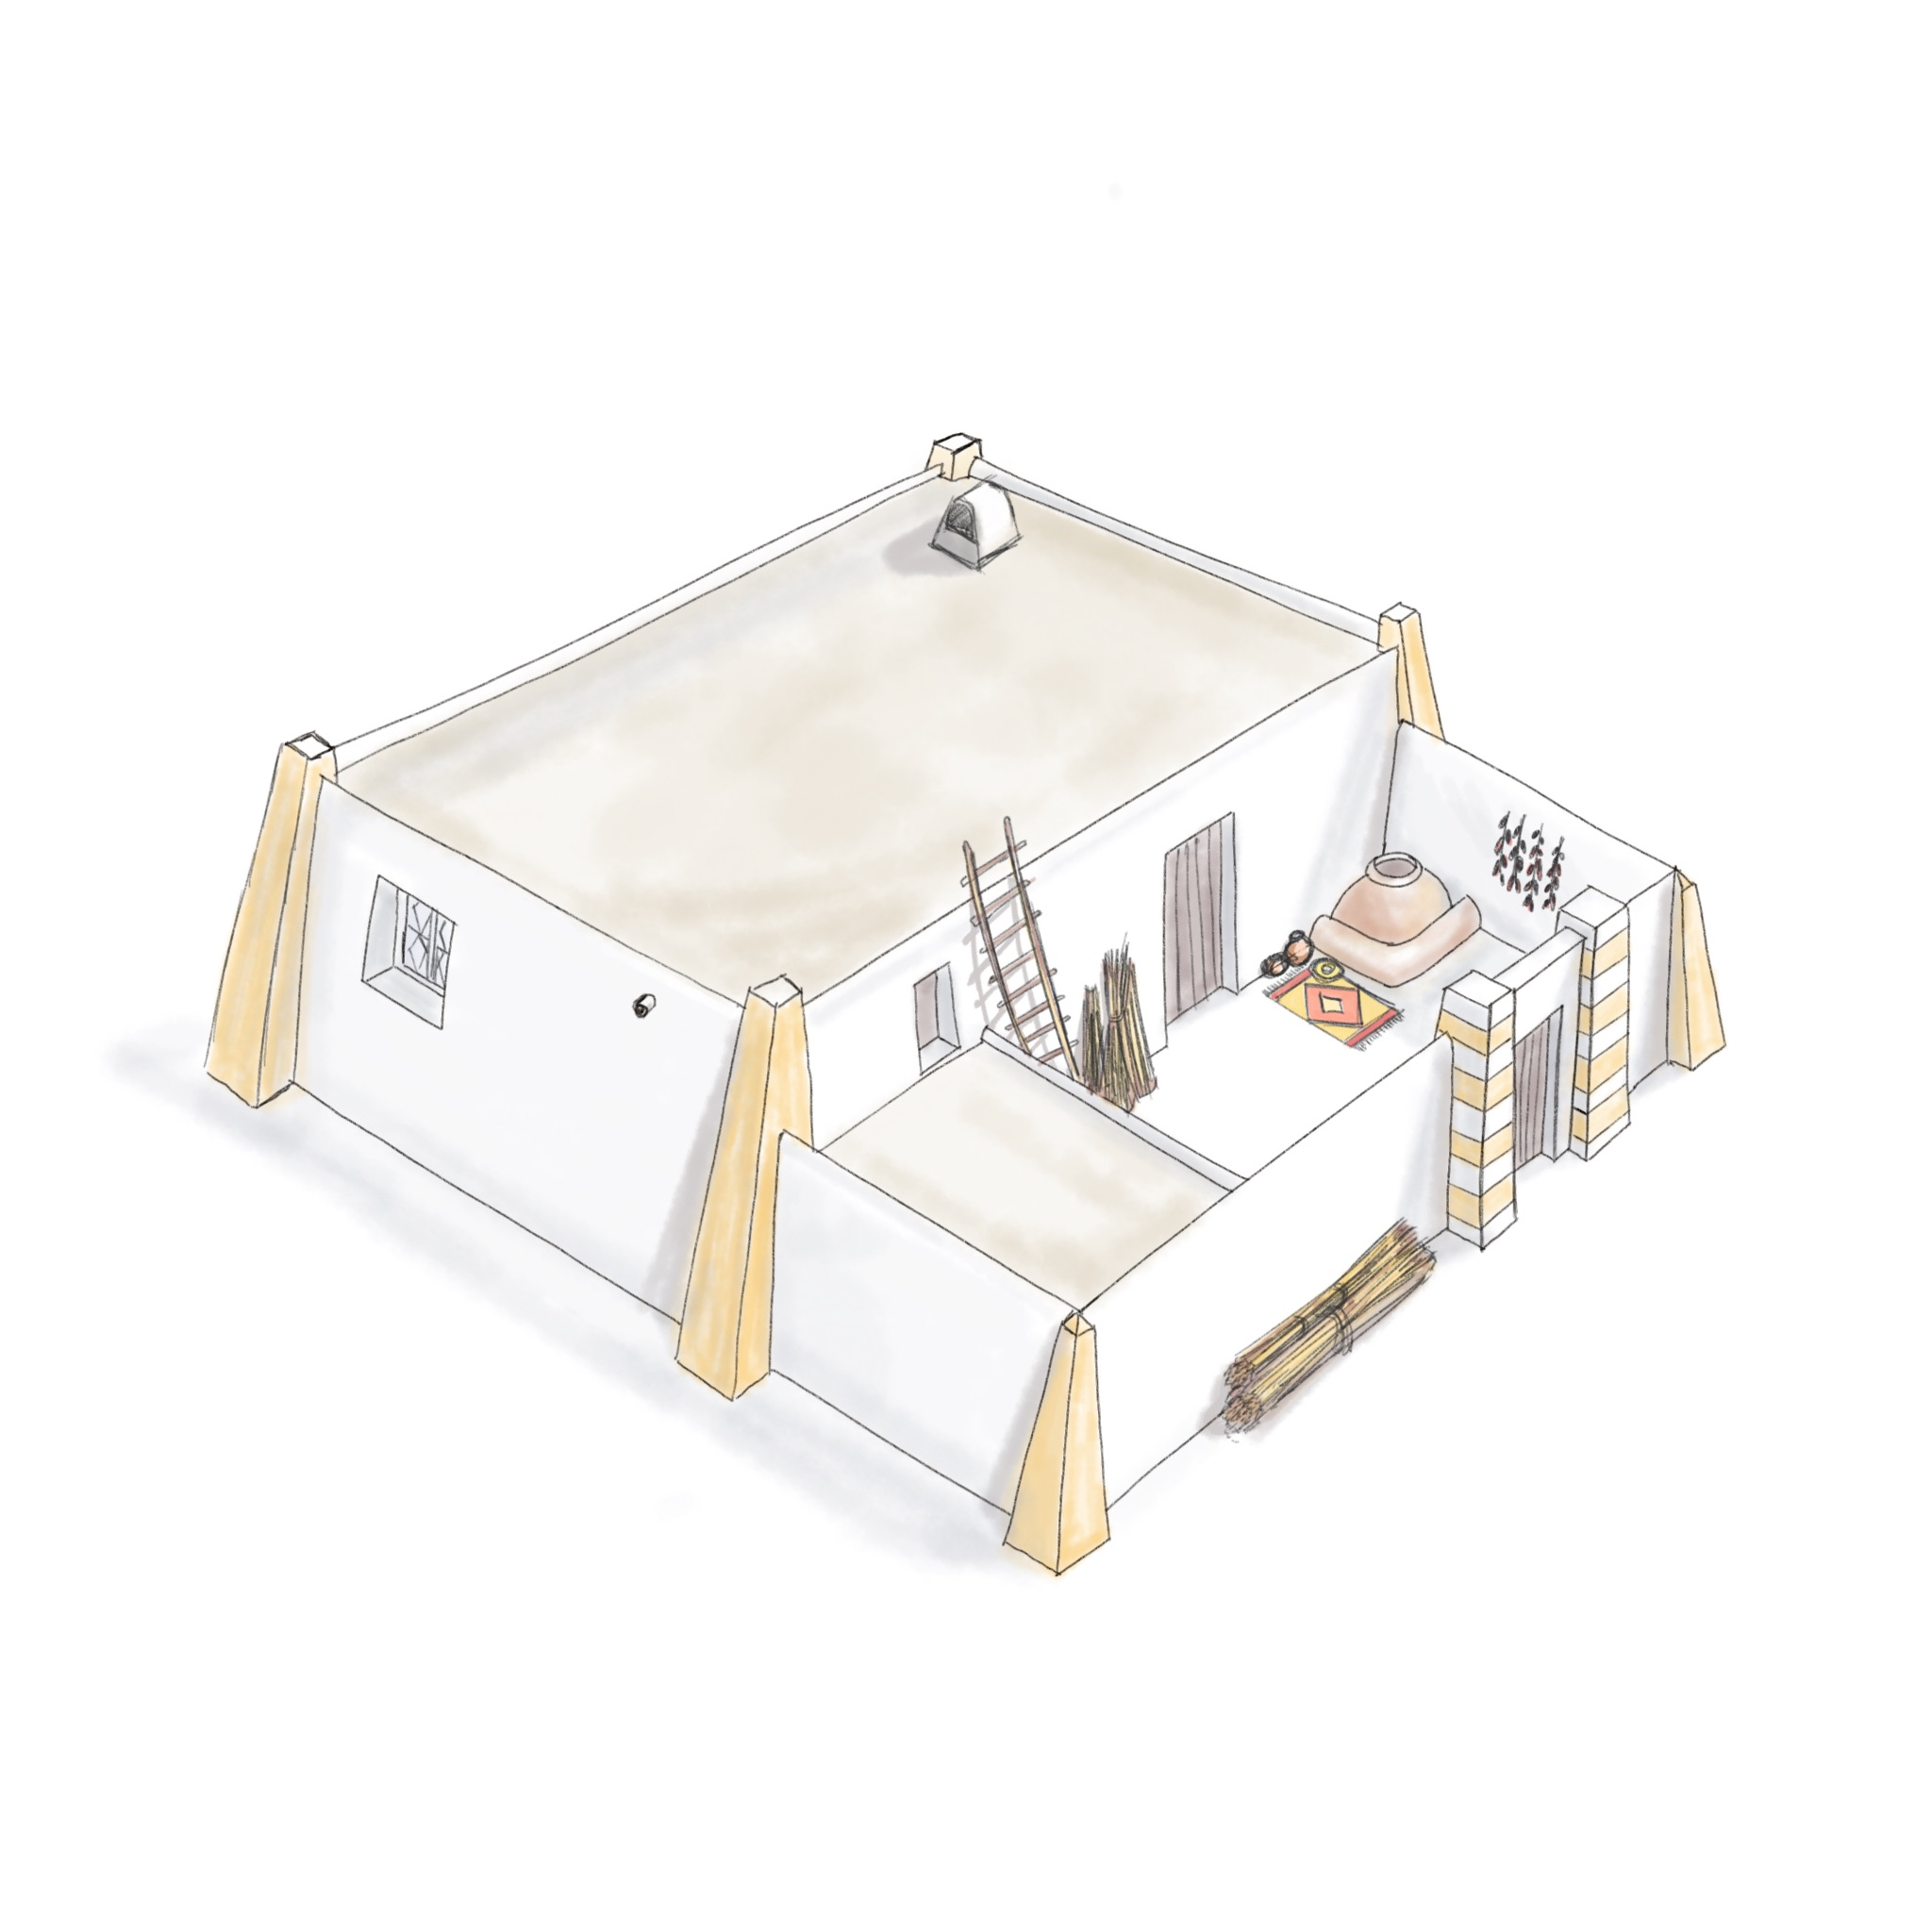
\includegraphics[width=\textwidth]{img/house/juli51_common_house}
	\caption{Common House by @Juli51}\label{fig:common_house}
\end{figure}

\paragraph{About the House Sketch \ref{fig:house_sketch}:} I made a quick sketch of a Meroitic house based on the layout you presented in your second work, "the common house" \ref{fig:common_house}. I adjusted the design, to incorporate Kushitic architectural elements. Like a narrow hall with barrel vault roof. I also made the windows facing outward very small, and placed them high in the wall, so that intruders can't crawl through them. I made the roof of the smaller structure out of palm branches, supported by a light wooden frame. This provides shade, but allows smoke to leave the room, which is how they made their kitchens. It makes for good cooking. I also added some improvised decoration to the front wall 

\begin{figure}[H]
	\centering
	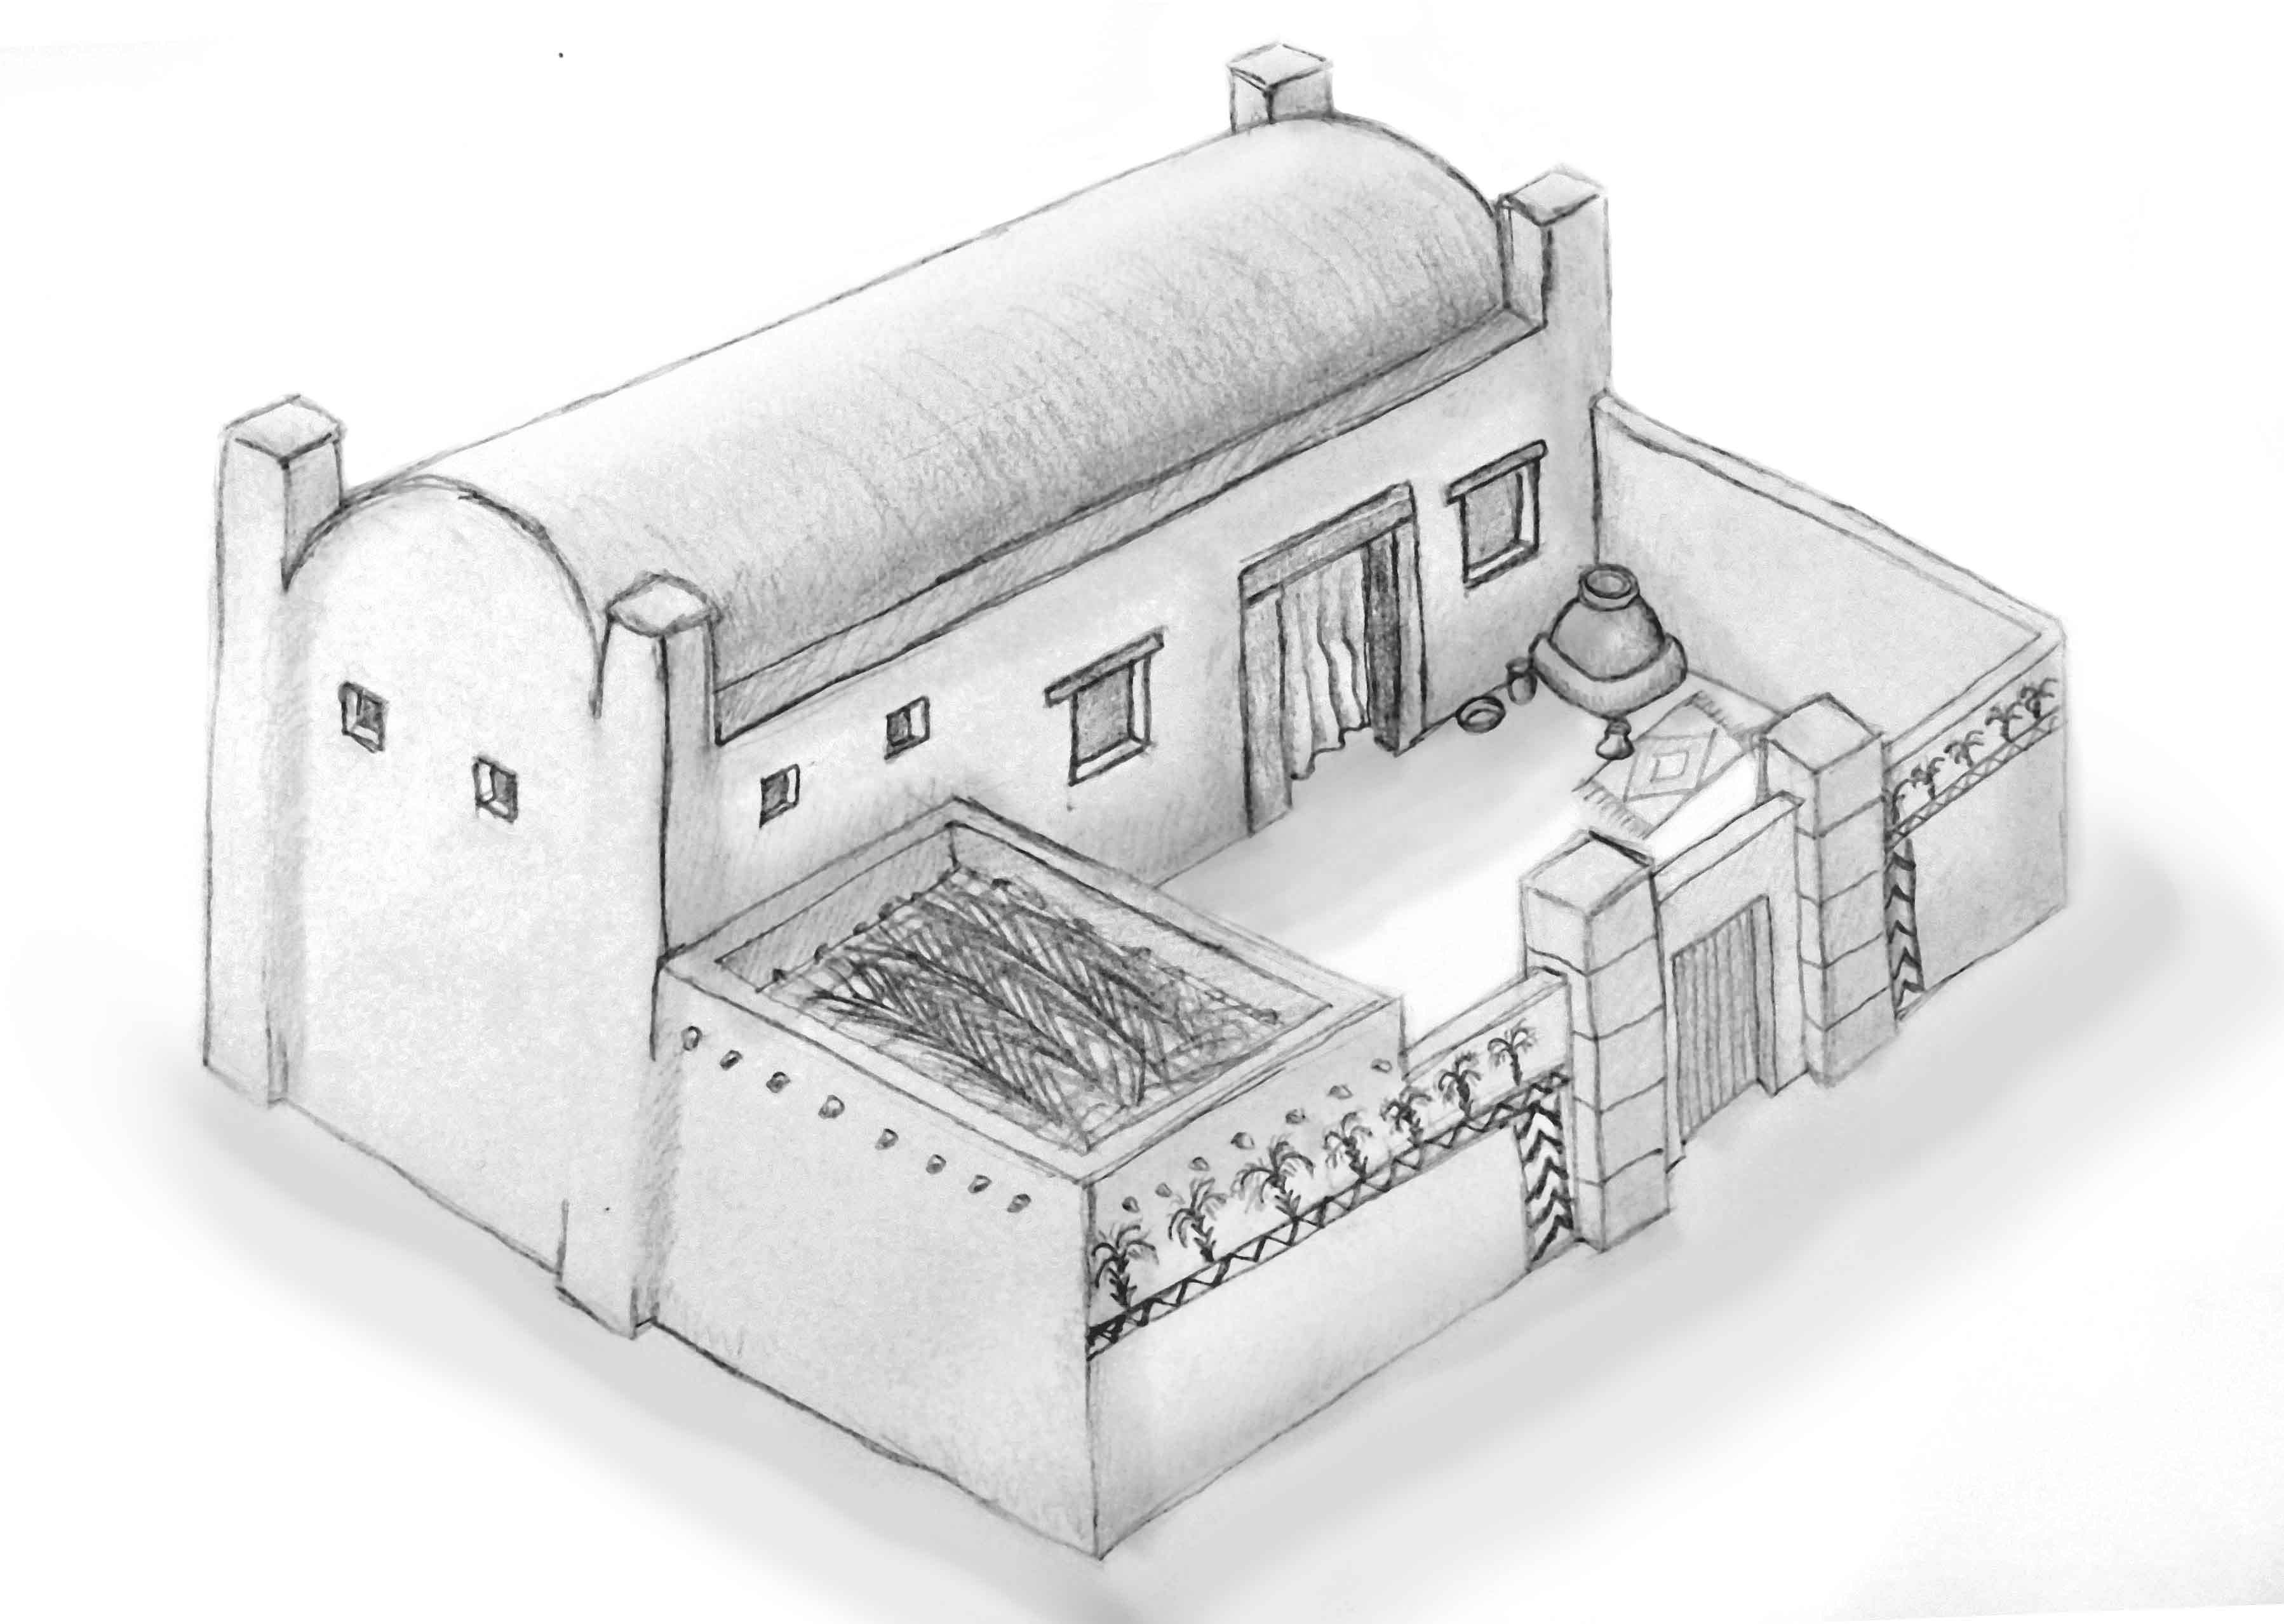
\includegraphics[width=\textwidth]{img/house/sundiata_house_sketch}
	\caption{House Sketch by @Sundiata}\label{fig:house_sketch}
\end{figure}

\section{Units}

\subsection{Chariot}

\section{Common Misconception}

\subsection{War Elephants}

Short answer: no, they did not use them.

TODO Long answer

\subsection{Nubia And Related Terms}

Nubia and related terms: The term is quite confusing at times because it refers to many possible things: 1) A geographical area generally identified as the area between the 1st and the 6th cataracts. 2) Nubian people, who descend from the Noba, 4th century Nomadic settlers on the Nile between the 1st and 3d cataract. 3) Nuba people, a distinct collection of Southern Sudanic tribes, mainly in Kordofan. 4) Nubian languages, refers a Nilo-Saharan language group, spoken by the descendants of the Noba, as well as Nuba people.\\  

The Kushites pose a serious question mark here, because Kushites don't seem to be Nubian at all. They didn't speak a Nubian language, they spoke Meroitic (neither Nilo-Saharan, nor Cushitic). Nubian, in ancient Egypt, seems to refer mostly to the people directly to the south of them, and those people formed a buffer between the Egyptians and "the wretched Kush". Kushites often warred against, and subjugated the people of Lower nubia. An additional point is that Kushite territory stretched far beyond Nubia. Some of it's most important cities weren't in Nubia at all, but to the south of it. Meroe itself lies between the last two cataracts. 

\section{Weaknesses and Strengths}

All this reading has made a few things clear to me. The Kushites had particular strengths and weaknesses relevant to the game-play of 0AD.

Weakness:

\begin{itemize}
	\item Weak armor: Basic units barely used armor. Special units, champions and heroes have (quality) quilted cotton and scale armor, but they should be relatively expensive.
	\item Weak navy. Apparently no real seafaring capability (which means they’d be a weak choice for an island map). But they did have boats, and transport of troops, and basic naval defense is a definite yes. Weak boats can be compensated with garrisons of archers, firing volleys of flaming arrows (fig. 7a).
	\item Weak siege equipment: Only cursory mention of siege equipment and tactics, which include ladders, ship-masts, sapping attacks on walls, but also siege towers and battering rams.
\end{itemize}

Strength:

\begin{itemize}
	\item Infantry should have a speed bonus, because low armor makes them faster (and cheaper)

	\item Their cavalry should be particularly strong and fast. Highly desired by the Egyptians and Assyrians, the specific breed of Kushite horses was large, fast and strong. I believe it is the ancestor to the rare Dongola, or Dongolawi horse, an important breed throughout the greater Sudan in later times (disregard Wikipedia on this one. Their page dismisses the Sudanic origin of this breed, apparently based on the axiom that horses were introduced to Sudan in much later times. By now we know they were being bred by the 2nd millennium BCE, but this isn’t common knowledge I guess. In addition, the page fails to distinguish, or even identify the unique physical features of this breed. The author seems to be conflating barb and Arab horses with older African breeds).

	\item Fast chariots (drawn by two horses), shooting accurate volleys of arrows. Perfect for hit and run tactics.

	\item Large-scale food production, due to irrigation and cattle herding. Allows recruiting many, fast and cheap units early in the game, ideal for early raiding.

	\item Strong buildings and defenses. Thick walls of cut stone, dry-stone or fired brick. Mud-brick foundations provide a certain plasticity, which in turn ensures the stability of larger structures.

	\item Strong weapons. Early iron (steel) production gives them strong swords, spears and arrow tips. Maybe they should have a weak defense, but a strong attack.

	\item They were world renowned for their archery skills for several millennia. They should be the most accurate archers in the game. Even in later times, Heliodorus of Emesa mentions their “unerring skill in hitting their target, their adversaries’ eyes”. This was repeated by the invading Arabs of the Rashidun Caliphate, who called them “pupil smiters”, and were forced to retreat from Sudan with many eyes lost (battle of Dongola).  
\end{itemize}

\chapter{Art and Design}

\section{Color Palette}

\section{Textures}

\chapter{Miscellaneous}

\section{Licenses}

\begin{itemize}
	\item Code: GPL v2
	\item Documentation: GPL v2 (excluding images)
	\item Images: Creative Commons
	\item 3D-Models?
	\item Sound?
\end{itemize}

\chapter{The Kingdom of Kush: A proper introduction}

\begin{center}
\textit{“Oh Great God, swift one. Who comes to him who calls. Watch my sister for me, the woman born in the same womb as me. Do for her as I have done for you. Spontaneous miracles that cannot be denied. Elevate her children and make them prosper, even as you did for me.”}\\[12pt]

\noindent
-From Taharqa’s prayer to Amun, at his temple in Kawa-
\end{center}

\begin{figure}[H]
	\centering
	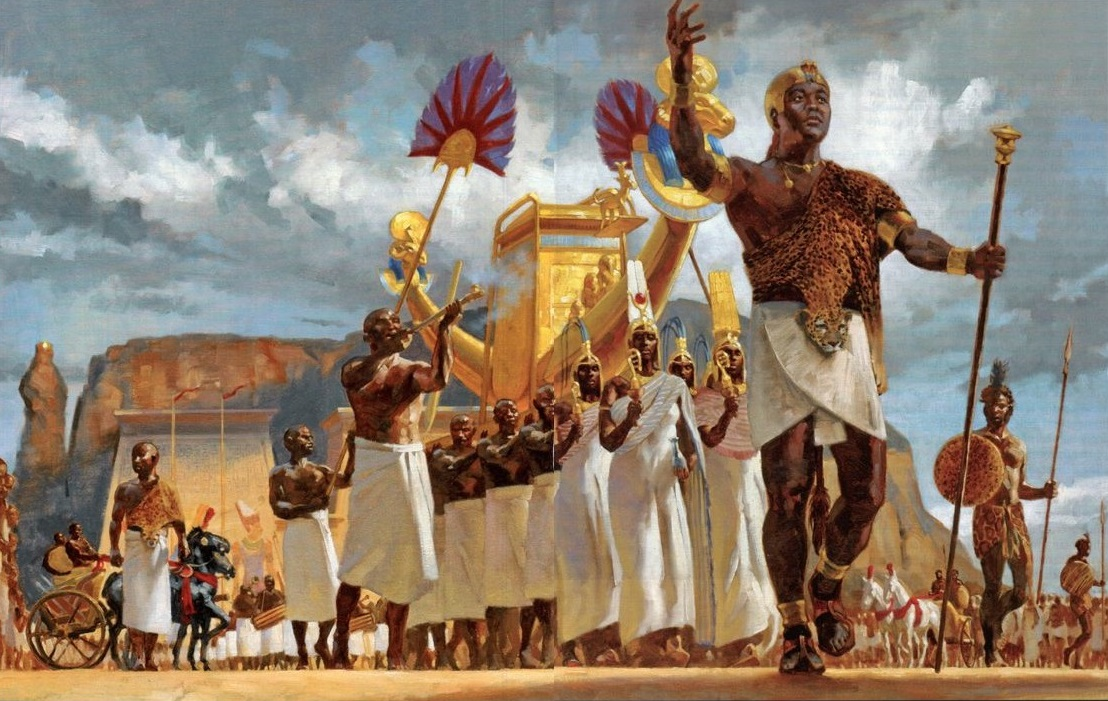
\includegraphics[width=\textwidth]{img/taharqa_pharaoh}
	\caption{Taharqa, pharaoh of the 25th dynasty and father of the later Meroe period, at the temple of Amun in Napata. The holy mountain Jebel (Gebel) Barkal is in the background.}
\end{figure}

Often misunderstood, and even more often overlooked, Kush was a major center of power in the ancient world. Its deserts and its armies were the southern frontier for many classical civilizations. Its gold and ivory were prized throughout the Mediterranean and the Middle East. Its trade routes connected Africa to the rest of the world and its mercenaries served as far as Greece. It’s rulers, many of them powerful queens, known as Kandakes, ruled in the style of the Pharaohs of the New Kingdom. City builders, administrators, craftsmen and artists, ironworkers, priests, warriors, farmers, cattle herders and horse breeders. Builders of pyramids. The bowmen of Nubia. Who where these Kushites, and why would they be such an invaluable addition to 0 A.D.?

\begin{figure}[H]
	\centering
	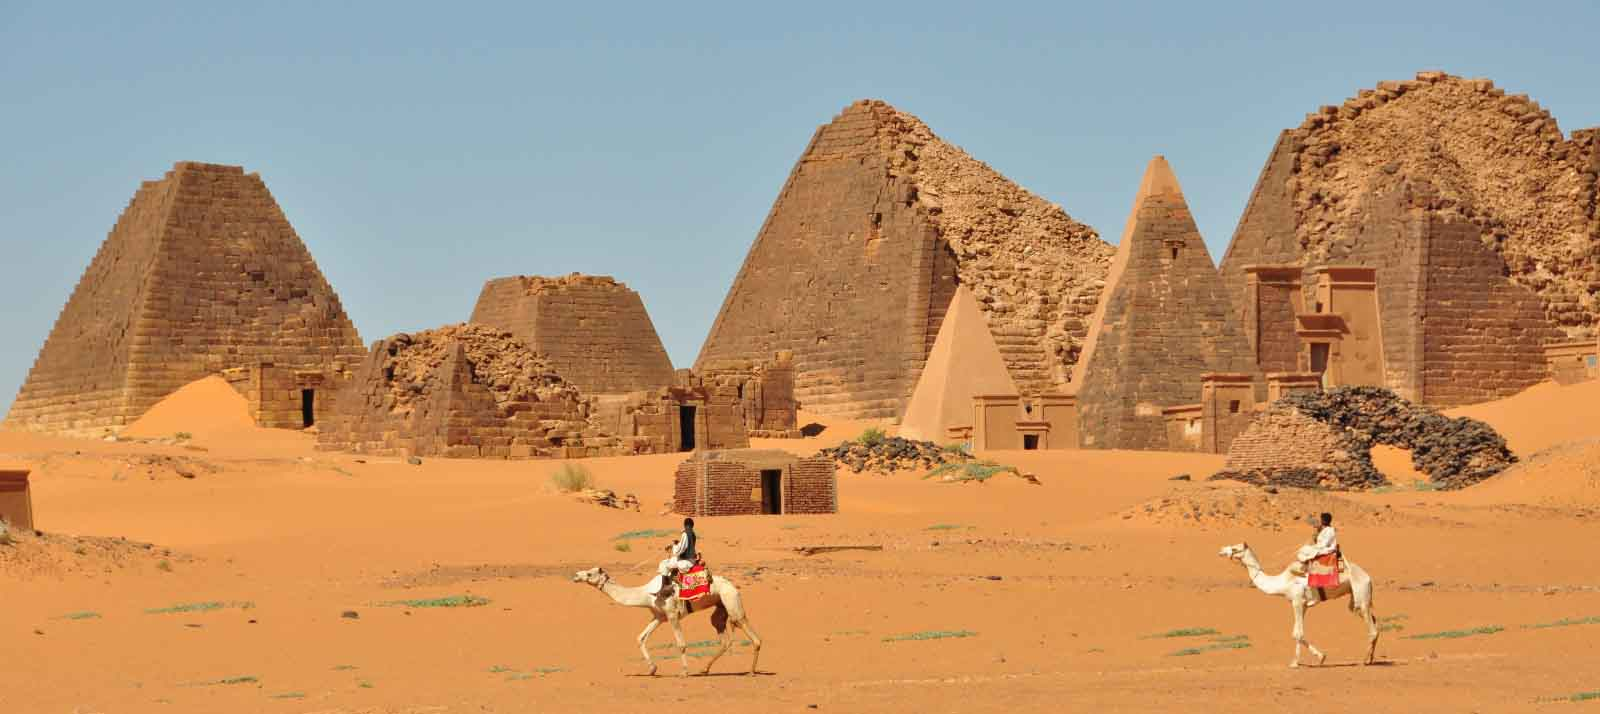
\includegraphics[width=\textwidth]{img/meroe_pyramids}
	\caption{Some of the Iconic Nubian pyramids, at Meroe. Between the 8th Cenury BCE and 350 A.D., 255 pyramids were built by the Kushites, at El Kurru, Napata, Meroe and Nuri.}
\end{figure}

Because the Kushites have not yet been properly introduced, I will attempt to provide you with a thorough, yet concise, illustrated analysis of Kushitic history, outlining their origin and environment, culture and religion, architecture, economy and military. As well as contextualizing them in a broader Mediterranean and Middle Eastern world, around the time frame of 0 A.D., including the prolonged wars they waged against several civilizations already featured in the game. Because of the lack of credible and historically accurate representations of these people in popular culture, I have spent some time, gathering a rich collection of historically accurate and relevant images, focused on important archaeological sites, and accurate reconstructions of houses, monuments, cities and the people and attire of various classes and backgrounds within Kush. If any attempt is made to represent “The Kingdom of Kush” in 0 A.D., the images provided in this introduction can provide the backbone for models of buildings and units, as they represent some of the most historically accurate images available on this civilization.

\begin{figure}[H]
	\centering
	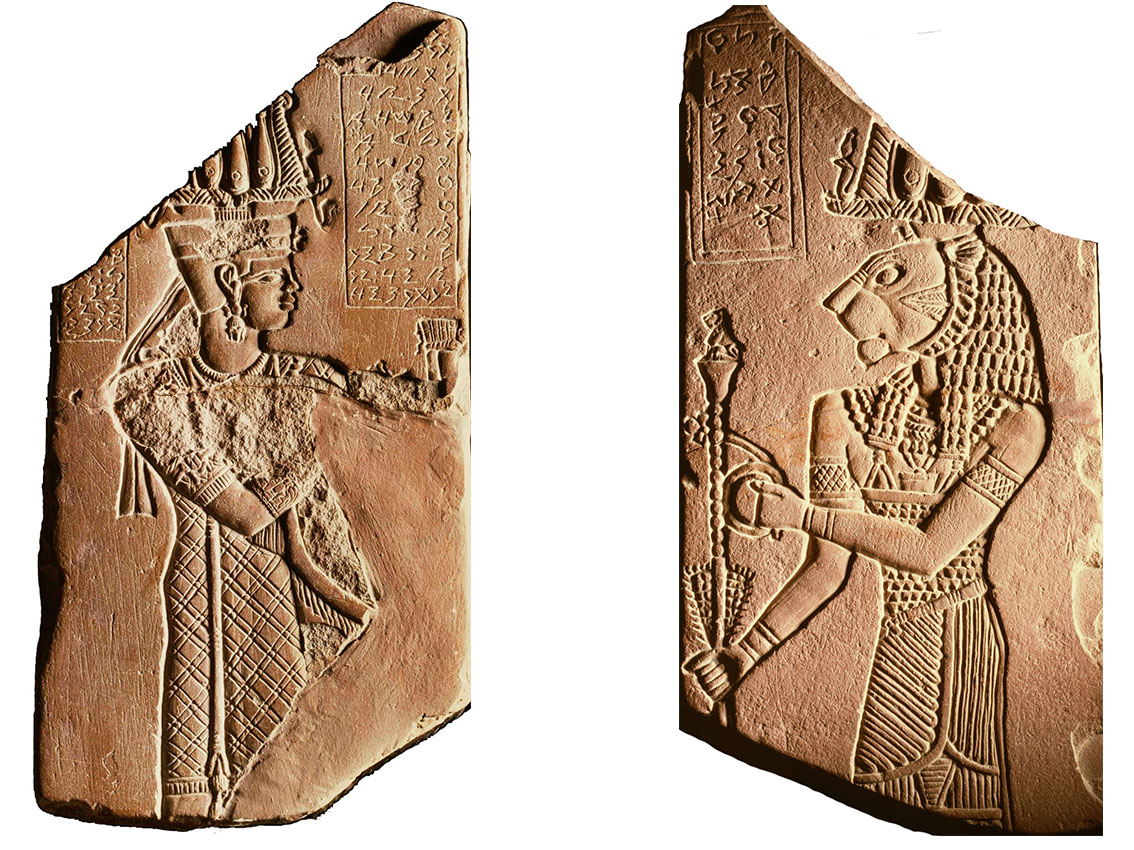
\includegraphics[width=\textwidth]{img/king_tanyidamani_and_apedemak}
	\caption{King Tanyidamani and Apedemak, the god of war and fertility, on a votive plaque from the Naqa kiosk.}
\end{figure}

\section{Indentifying Kush}

Kushites are known and referred to by a number of names, sometimes confusing the casual reader trying to find out more about these people. The following names are used interchangeably: “Kush”, or “The kingdom of Kush”, “The Kushitic empire”, “Napatans”, “Meroites”, “The Meroitic Empire” or more commonly, but less precisely, “Nubia”, or “the Nubians”. Egypt’s fearsome southern neighbor. This is Herodotus’ Aethiopia (Ethiopia). It must not be confused with the modern day country of Ethiopia, which lies to the south of ancient Kush. Neither should they be confused with the “Kushans” of Bactria and India. The Kingdom of Kush was centered in modern day Sudan. More specifically on the Butana step, a vast, semi-arid, seasonal savannah, flanked by the Nile and the Blue Nile to the West, and the Atbarah River to the East. There, people took advantage of seasonal rainfalls to engage in large-scale agro-pastoralism. Mainly cattle herding and the cultivation of barley, wheat, sorghum and millet, along with cash crops like cotton and dates. In 450BCE Herodotus correctly identified the capital as Meroe, an ancient site that was used for royal burials as early as 890BCE. Situated between the 5th and the 6th cataract on the Nile, Herodotus called it a “great city... said to be the capital of the other Ethiopians”.

\begin{figure}[H]
	\centering
	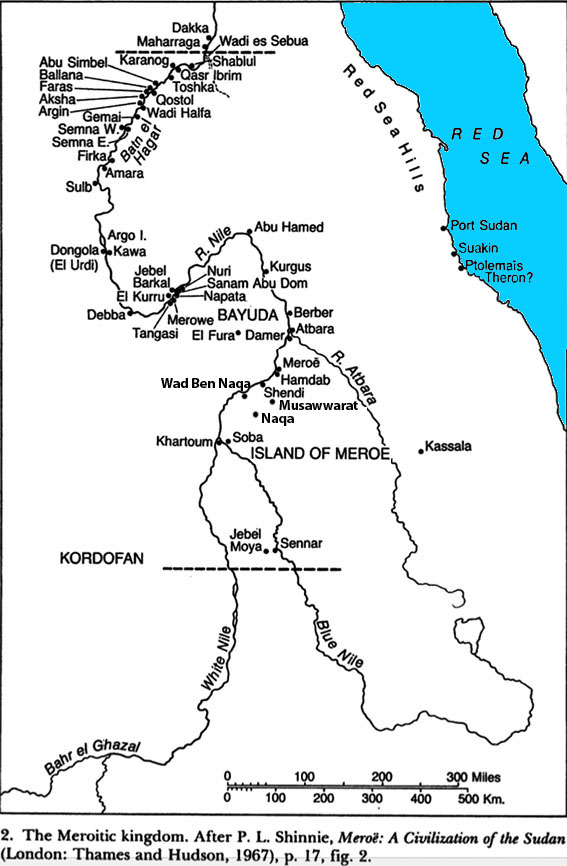
\includegraphics[width=\textwidth]{img/map_of_kush}
	\caption{A map of Lower, Upper and South Nubia, in modern day Sudan. The core of Kushite influence stretched about a thousand km, from the first cataract around Maharraqa (traditionally the Roman frontier), to Jebel Moya.}
\end{figure}

\section{Early History: Kerma and Napata}

\textbf{(Before the time frame of 0 A.D.) c. 3500BCE - 590BCE}\\

The Kingdom of Kerma is the first expression of Kushite culture. The Pre-Kerma period, beginning around 3500BCE, saw the development of the earliest known, dense settlement patterns in Sub Saharan Africa. By 2500BCE Kerma emerged as a regional center, and by 1700BCE the city of Kerma had an estimated population of over 10.000 people. It boasted monumental buildings and a system of thick defensive walls, miles of irrigation canals and engaged in long distance trade. It was the seat of a centralized state. The first of many in Sudan. 
 
\begin{figure}[H]
	\centering
	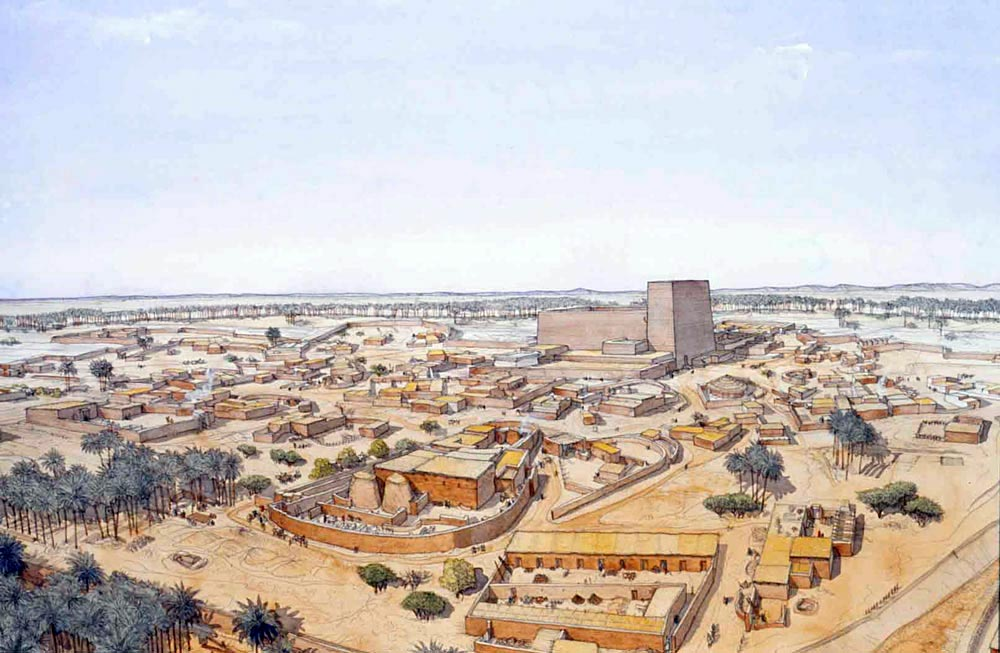
\includegraphics[width=\textwidth]{img/central_kerma}
	\caption{A view of central Kerma around 2000BCE. The large structure in the center of the town, presumably a temple, is called The Western Deffufa. It's impressive ruins still stand today. This image is based on the archaeological surveys revealing the town plan in relative detail.}
\end{figure}

The Kingdom of Kerma is attested in Egyptian records as Kush (k3š), as early as the Middle Kingdom, and its riches had been prized since the Old Kingdom. Then, starting with Senusret I, and particularly Senusret III of 12th Dynasty, Egypt gained its first permanent foothold in Lower (northern) Nubia, with the establishment of massive forts, such as Buhen in c. 1860BCE. By the 13th dynasty, Egyptian power waned, the forts were abandoned and Lower Nubia was reoccupied by Kush. By c. 1550BCE Kerma was strong enough to challenge Egypt itself, formed an alliance with the invading Hyksos from the north, and raided deep into Upper Egypt. These events almost brought about a premature end to Pharaonic Egypt, and led to the Second Intermediate Period. Curiously, Nubian bowmen served as mercenaries (the original Medjay), in Kamose’s campaign against their former Hyksos allies. 

\begin{figure}[H]
	\centering
	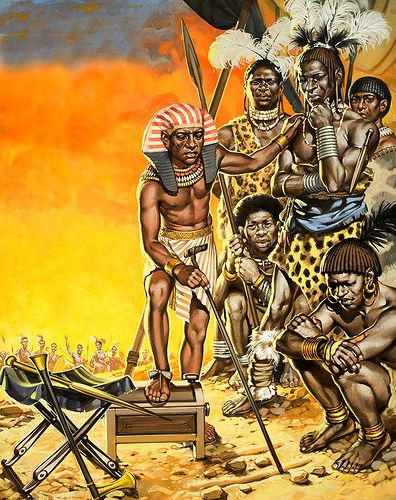
\includegraphics[width=\textwidth]{img/pharaoh_kamose_battle_plan}
	\caption{Pharaoh Kamose revealing the battle plan to his Kushite allies, during his "war of liberation" against the Hyksos.}
\end{figure}

Under Kamose, and the subsequent reestablishment of Egypt under the New Kingdom with Amenhotep I and Thutmose I, Kush was invaded several times, and Kerma was destroyed. For the next 500 years, upper and lower Nubia effectively became increasingly Egyptianised colonies, though the relationship was often of a symbiotic nature. 

\begin{figure}[H]
	\centering
	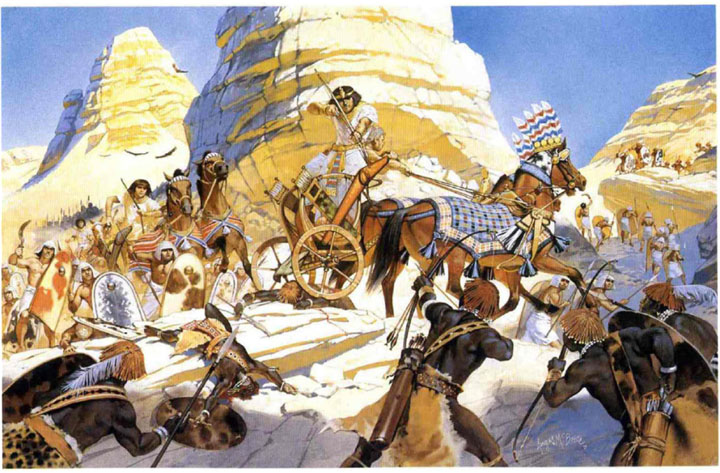
\includegraphics[width=\textwidth]{img/new_kingdom_battle}
	\caption{A New Kingdom Pharaoh campaigning in Lower Nubia.}
\end{figure}

In the 15th century BCE, Thutmose III established a small temple in Nubia at the foot of Jebel Barkal, a modest, lonely mountain rising steeply from the flat desert floor surrounding it. It was said to be the southern home of Amun, and marked Egypt’s southern most expansion. The existing town, now called Napata, was to become one of the most important centers of Kush. As it’s religious capital, it became the seat of the cult of Amun. Around 1075BCE, the New Kingdom collapsed, and the Egyptianised people of Kush set up an independent kingdom, centered on Napata. This ushered in the Napatan period.\\

By 721 BCE, the Napatans had become so powerful, that their king, Kashta, invaded Upper Egypt and occupied Thebes. His successor, Piye, completed the conquest, and conquered one of the largest empires the Nile Valley had ever seen. Piye, Shabaka, Shebitku, Taharqa and Tantamani all ruled Egypt, as well as Kush, as pharaohs of the 25th dynasty, also known as the “Nubian Dynasty” or the “Kushitic Empire”. They saw themselves as the custodians of Egyptian culture and religion. Piye built the first pyramid the Nile Valley had seen in over 500 years, a tradition the Kushite kings continued in to the 4th century A.D. They initiated major restoration projects on the ancient temples, and built many new ones, reinvigorating Egyptian traditional religion (especially the cult of Amun), as well as collecting tribute from powerful states in the Levant and expanding their military activity as far north as Judea.   

\begin{figure}[H]
	\centering
	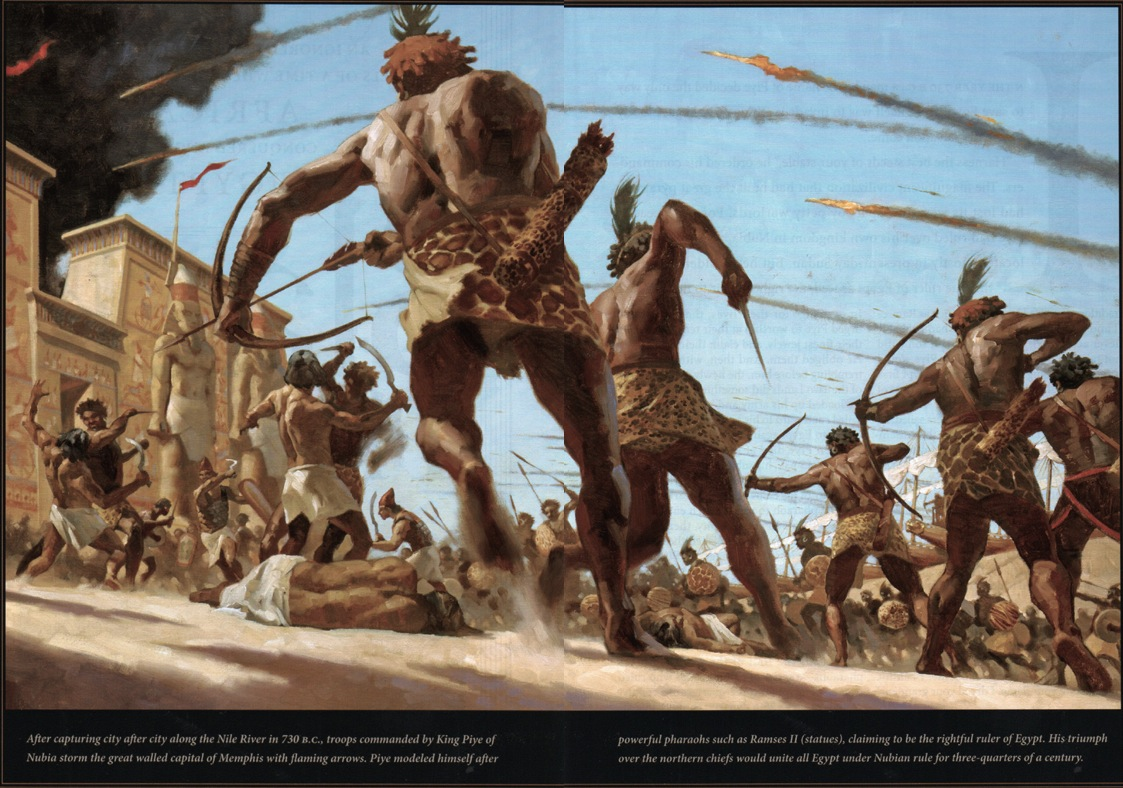
\includegraphics[width=\textwidth]{img/piye_troops_take_memphis}
	\caption{Piye's troops take Memphis, the northern capital, thereby unifying all of Egypt and all of Kush.}
\end{figure}

\begin{figure}[H]
	\centering
	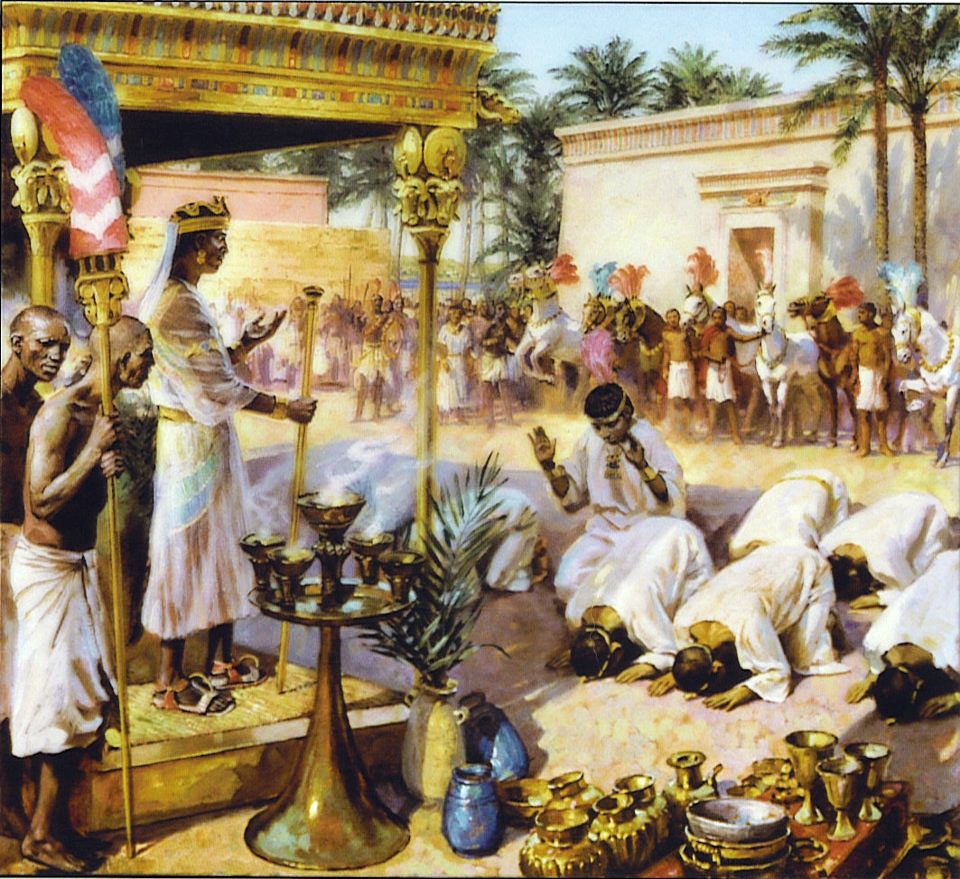
\includegraphics[width=\textwidth]{img/piye_tribute}
	\caption{The Pharaoh Piye receiving tribute from Egyptian royals.}
\end{figure}

Growing tensions over Kushite activity in the Levant, led to a series of devastating wars with the Neo-Assyrian Empire beginning in 677BCE. In 671BCE, Taharqa fought running battles with the armies of Esarhaddon from the Sinai to Memphis, but was defeated, and fled to Thebes. Taharqa’s wife (and/or sister) and son, were both captured and taken to Nineveh. Tantamani restored Kushite rule in Egypt to some extent, but by 656BCE, Psamtik I of the Saite Dynasty took control of Thebes, ending the Kushite presence in all of Egypt. Psamtik II, with the participation of Greek mercenaries, campaigned in Lower Nubia. By 590BCE the Kushite seat of authority was shifting towards the more southern Meroe, eclipsing Napata, and giving rise to a distinctively more “Africanised” Meroitic culture. The Neo-Assyrian Empire collapsed in 609BCE, and was absorbed by the Persian Achaemenid Empire under Cyrus the Great. His successor, Cambyses II, successfully conquered Egypt in 525BCE, after which he attempted the conquest of Kush. He was met with catastrophic failure, possibly because of the difficulties associated with marching an army through the desert.

\begin{figure}[H]
	\centering
	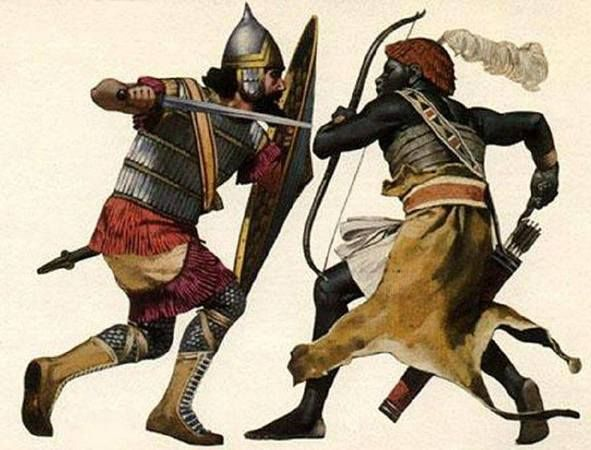
\includegraphics[width=\textwidth]{img/assyrian_vs_nubian}
	\caption{An Assyrian and a Nubian fight it out, in one of many battles fought during the Assyrian invasion of the Levant and Egypt.}
\end{figure}

By all accounts, the Pharaohs of the 25th dynasty, especially Piye and Taharqa, are to be considered the fathers of the later Meroitic period, and its subsequent rulers. The Kings of Meroe went to great lengths to preserve the Egyptiansed customs they inherited. But neither did they shy away from developing their own, independent culture, religious practices, writing systems, architectural styles, aesthetic principles, military systems and trade networks. They also incorporated Greco-Roman, Ptolemaic, Persian and Indian influences. Combined with their close proximity to very warlike, sometimes nomadic, African tribes (like the Blemmyes) and the assimilation of many of these tribes in to a greater Kushite state, demonstrate a level of social complexity rarely seen in this region in later times. The complex interaction of many peoples, cultures and influences, increasingly transformed Meroe in to a uniquely African civilization. It is this later expression of Kushite culture, during the Meroitic period that we shall examine further. Starting around 590BCE, when Meroe started eclipsing Napata, and ending with the Axumite invasions of Kush, around the 330's AD, the Meroitic period spans the entire length of 0 A.D.’s timeframe and beyond.

\begin{figure}[H]
	\centering
	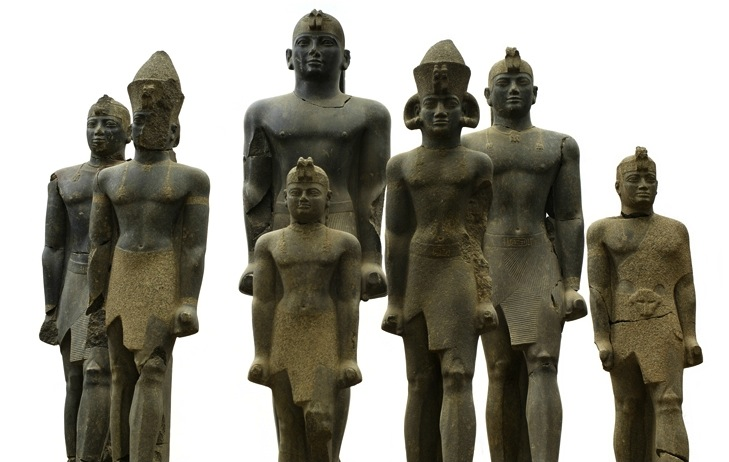
\includegraphics[width=\textwidth]{img/naptan_kings}
	\caption{In a pit, close to Kerma, the broken statues of a number of Napatan Kings were uncovered, including some of the 25th dynasty, and later Kings. The known kings are: Taharqa, Tanoutamon, Senkamanisken, Anlamani and Aspelta. This find, along with others, show that Kerma was still important, long after its destruction, and it also shows a clear continuity from the 25th dynasty to later Kushite kings.}
\end{figure}

\section{The Meroe Period}

\textbf{(During the time frame of 0 A.D.) c. 590BCE – 330AD}\\

Napata was essentially a southern expression of classical Egyptian culture. In fact, it can be said that during the height of the Napatan 25th dynasty, the material culture of Nubia and Egypt become indistinguishable. The same cannot be said for Meroe. The move to Meroe symbolizes a break from the strict, Egyptian character of the earlier Napatan Period, and saw the mixing of African, Egyptian, Middle Eastern and Mediterranean influences. Napata remained one of the most important cities in Kush, though, and the Kings of Meroe built new temples and palaces, maintaining its religious authority throughout the Meroitic period.

\begin{figure}[H]
	\centering
	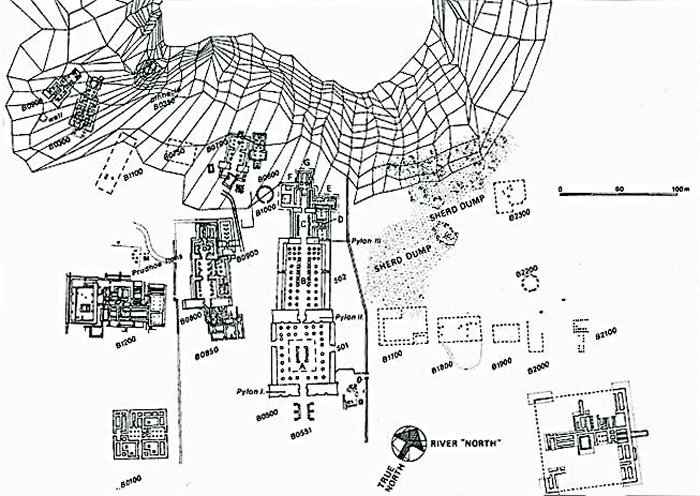
\includegraphics[width=\textwidth]{img/napta_temple_district}
	\caption{Detailed plan of excavation results in Napata, showing the central "temple district", with many temples to various gods and even 2 visible palaces.}
\end{figure}

\begin{figure}[H]
	\centering
	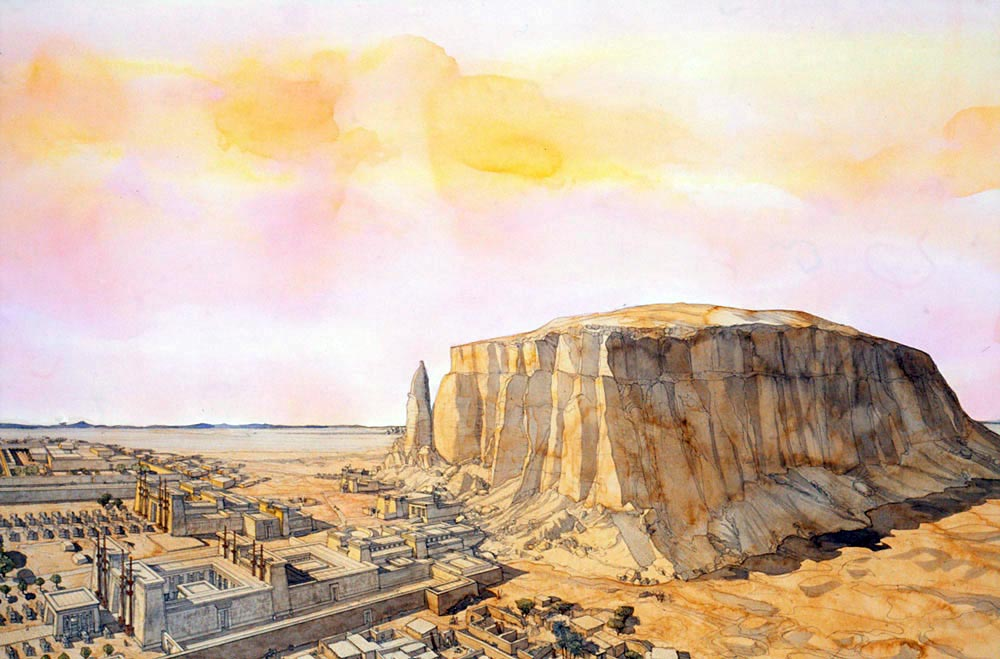
\includegraphics[width=\textwidth]{img/holy_mountain_jebel_barkal}
	\caption{Napata in it's full glory around the 1st century BCE, infront of the holy mountain, Jebel Barkal. King after King commissioned restorations and new temples. Even after the move to Meroe, many kings continued to be crowned here. This illustration stays true to archaeological reports on the site.}
\end{figure}

Possibly prompted by increasing hostility from Egypt and the Persians to the north, the more southern Meroe became increasingly important. Another possible reason for the move south, is that the Napatan Kings of Kush were trying to brake from the authority of the cult of Amun, the foremost religious authority in Kush, also centered in Napata. By moving the royal capital to Meroe, the society was secularized, and the Kings enjoyed a greater freedom than before. This move was completed by the time of Arakamani, identified with “Ergamenes”, of Diodorus Siculus’ Bibliotheca Historica, in the early third century BCE. According to Diodorus, the priesthood of Amun had the power to order the death of a king. Ergamenes (Arakamani), was the first King to brake from this tradition, when the priests ordered his death. He moved on Napata, ordered the massacre of the priests, and moved the royal burial grounds to Meroe, where many of the iconic Meroitic pyramids were built. Diodorus states that his strong will came from his instruction in Greek philosophy, probably related to the rule of the Ptolemies in Egypt. Regardless of the changing relationship between the kings and the cult of Amun, the worship of Amun remained important throughout Kushite history. Temples to Amun continued to be built in to the third century A.D., and the cult was still present during the Christianization of Nubia in the 6th century A.D. 



\end{document}
